% $Id$

\chapter{Block design fMRI dataset}
\label{sec:Block_design_fMRI_dataset}
\minitoc

This chapter will describe the steps necessary to perform a classification using PRoNTo. The dataset\footnote{Pre-processed (realigned and normalised) data from participant 1.} used in this chapter can be found in PRoNTo's website \url{http://www.mlnl.cs.ucl.ac.uk/pronto/prtdata.html} (data set 1) and the whole\footnote{Not pre-processed.} dataset is available in \url{http://data.pymvpa.org/datasets/haxby2001/}.

This fMRI dataset originates from a study on face and object representation in human ventral temporal cortex \cite{Haxby2001}. In this study, the subject was shown a set of grey scale images of 8 categories (faces, houses, cats, chairs, bottles, scissors, shoes and scrambled pictures), with 12 runs/blocks. Each image was displayed for 500 ms and was followed by a 1500 ms rest interval. This experiment consisted of a block-design of 9 scans of each category followed by 6 scans of inter-stimulus interval. Images were acquired with a TR of 2.5 s. The full-brain fMRI data consisted of 1452 scans/volumes with 40 x 64 x 64 voxels. The dimensionality of each voxel was 3.5 x 3.75 x 3.75 mm.

For simplicity, in this example we will use PRoNTo to predict if the subject is viewing an image of a face or a house based on the fMRI scans. We will classify the whole brain images using Support Vector Machines, using a leave one block out cross-validation scheme.

\section{GUI analysis}

We will first analyse the data using PRoNTo's GUI and then repeat the analysis using the {\tt matlabbatch} system.

To start, create a new directory in which to save the results of the analysis, then start up \matlab{} and type `prt' or `pronto' in the \matlab{} prompt (considering that the PRoNTo and SPM folders have been previously added to the \matlab{} path). This will open the main interface of PRoNTo (Figure \ref{fig:gui_main_screen}).

\begin{figure}[!h]
	\centering
		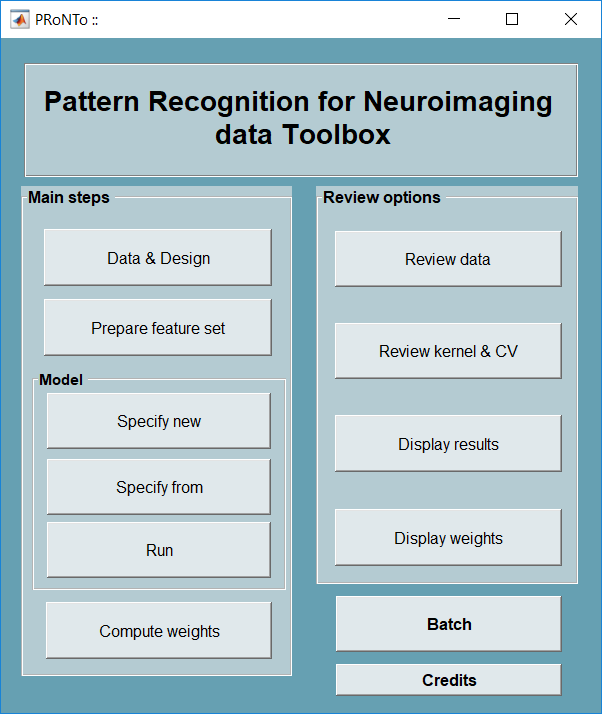
\includegraphics[scale=0.6]{images/Tutorial/v3/data_example1/gui_main_screen.png}
	\caption{Main interface of PRoNTo.}
	\label{fig:gui_main_screen}
\end{figure}

%--------------------------------------------------------------------------
\subsection{Data \& Design}

\begin{itemize}
	
	\item In PRoNTo's main window, click on `Data \& Design' and a new window will open, `Data and design' (Figure \ref{fig:gui_data_and_designs_blank}). Then, browse the directory in which to save the PRT structure (saved as `PRT.mat').
	
\begin{figure}[!h]
	\centering
			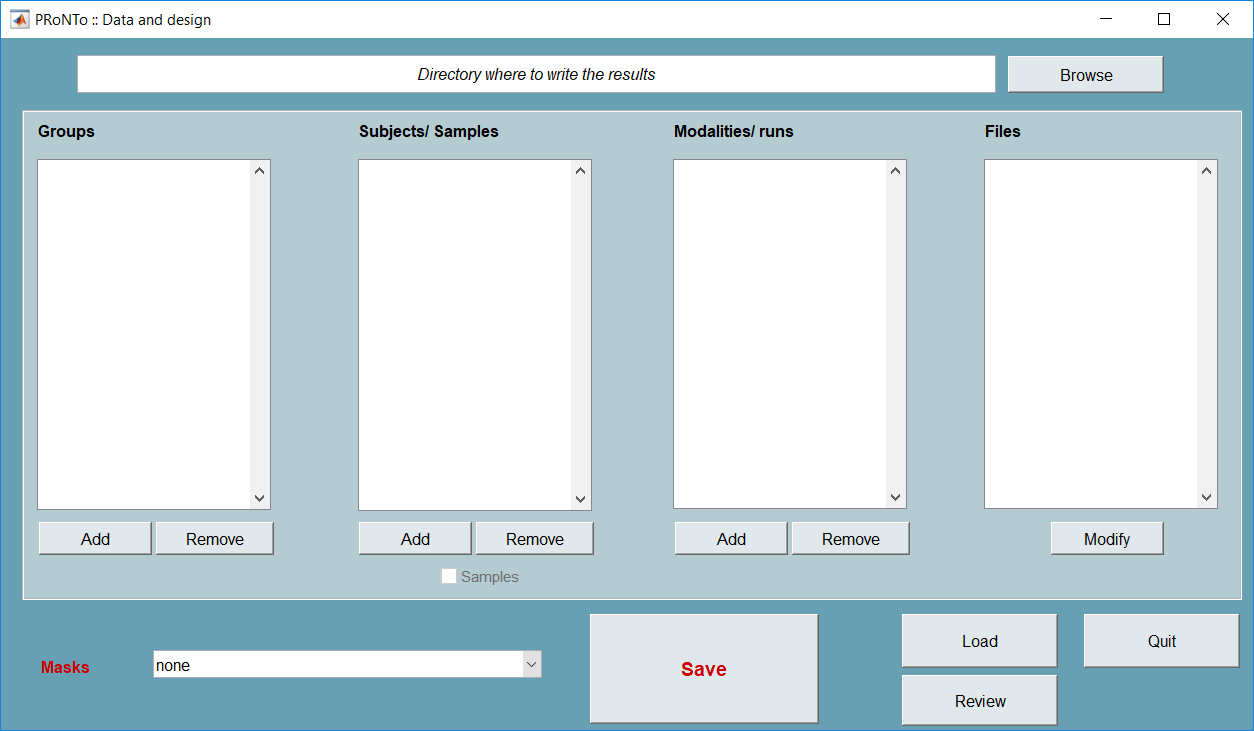
\includegraphics[scale=0.5]{images/Tutorial/v3/data_example1/gui_data_and_designs_blank.png}
	\caption{`Data and design' GUI.}
	\label{fig:gui_data_and_designs_blank}
\end{figure}
	
	\item In the panel `Groups', click on `Add' and provide a name to the group (we only have one group/subject), with no spaces or special characters, e.g. `G1'.
	
	\item Add a subject in the `Subject/Samples' option, e.g. `S1', and leave the `Samples' tick box below the panel unchecked. See Chapter \ref{chap:DataDesign} of the manual for more information on this option.
	
	\item In the `Modalities' panel, click on `Add' and provide a name to the modality, e.g. `fMRI'. The `Specify modality' GUI allows one to specify the format of the Data and the design of the experiment. In the `Data format', choose `nifti' (Figure \ref{fig:gui_data_and_design_modality_data_format}).  In the `Design' field, choose the option `Load SPM.mat' (Figure \ref{fig:gui_data_and_design_modality_specify_design}). This file is available with the Haxby dataset on PRoNTo's website\footnote{http://www.mlnl.cs.ucl.ac.uk/pronto/prtdata.html} inside the folder Haxby\_dataset/design/. Finally, in this case leave `Regression targets' as it is, in the `No targets' option.
	
\begin{figure}[!h]
	\centering
	\begin{minipage}[b][7cm][b]{0.5\textwidth}
  \centering
		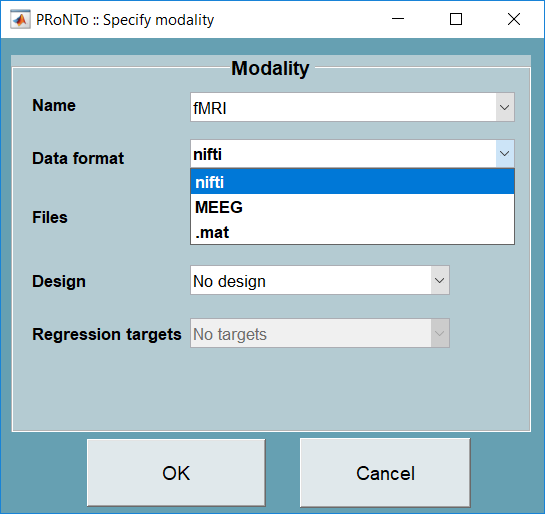
\includegraphics[scale=0.5]{images/Tutorial/v3/data_example1/gui_data_and_design_modality_data_format.png}
		  \captionsetup{width=0.8\linewidth}
	\captionof{figure}{`Specify modality' GUI. First we specify the format of our data (here nifti).}
	\label{fig:gui_data_and_design_modality_data_format}
\end{minipage}%
	\begin{minipage}[b][7cm][b]{0.5\textwidth}
  \centering
		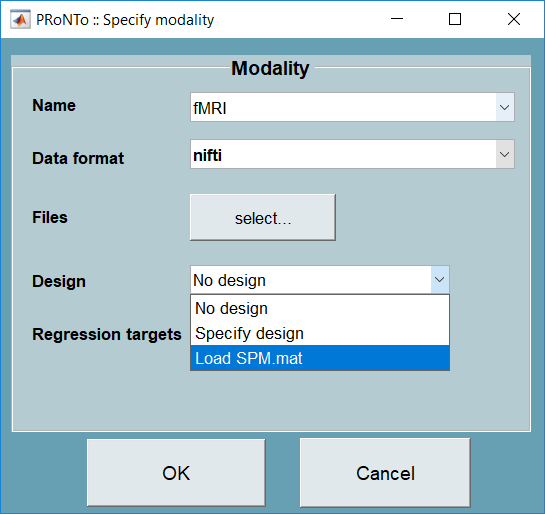
\includegraphics[scale=0.5]{images/Tutorial/v3/data_example1/gui_data_and_design_modality_specify_design.png}
		\captionsetup{width=0.84\linewidth}
	\captionof{figure}{`Specify modality' GUI. Here we load a specified design from an `SPM.mat' file.}
	\label{fig:gui_data_and_design_modality_specify_design}
	\end{minipage}
\end{figure}

	\begin{itemize}
	
		\item In case there is no `SPM.mat' file available to use, create a new design by selecting the option `Specify design'. Choose how many conditions you have, which in this case are 8 conditions (corresponding to the 8 categories of images). This will open another window that allows the user to write the names, onsets and durations of each condition (Figure \ref{fig:gui_data_and_design_modality_specify_design_2}). If the duration of each event is different, you must specify the duration of all events as shown in the figure above. If however the duration is the same for all events, specifying one value per class will suffice (Figure \ref{fig:gui_data_and_design_modality_specify_design_3}). The unit in which the onsets/durations are read in this case is `scans' and the interscan interval (TR) is 2.5 seconds. The design information (names, onsets and durations) can be found inside the `Haxby\_design.pdf' file in the Haxby dataset folder. 

	\end{itemize}
	
	
\begin{figure}[!h]
	\centering
	\begin{minipage}[b][7cm][b]{0.5\textwidth}
  \centering
		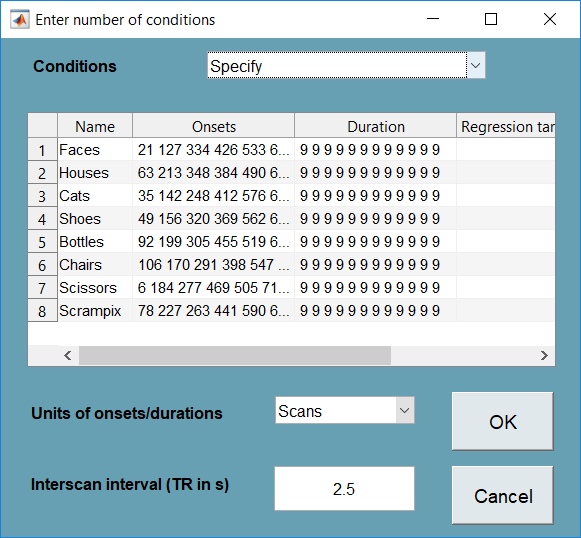
\includegraphics[scale=0.5]{images/Tutorial/v3/data_example1/gui_data_and_design_modality_specify_design_2.png}
		  \captionsetup{width=0.9\linewidth}
	\captionof{figure}{`Specify design' GUI to enter the conditions, the units of design, TR and covariates.}
	\label{fig:gui_data_and_design_modality_specify_design_2}
\end{minipage}%
	\begin{minipage}[b][7cm][b]{0.5\textwidth}
  \centering
		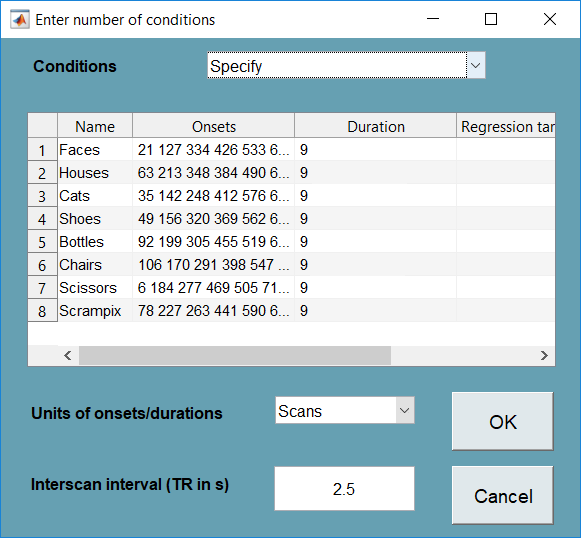
\includegraphics[scale=0.5]{images/Tutorial/v3/data_example1/gui_data_and_design_modality_specify_design_3.png}
		\captionsetup{width=0.9\linewidth}
	\captionof{figure}{If all events have the same duration, you can specify this with only one number.}
	\label{fig:gui_data_and_design_modality_specify_design_3}
	\end{minipage}
\end{figure}


% \begin{figure}[!h]
% 	\centering
% 		\includegraphics[scale=0.7]{images/Tutorial/gui_data_and_design_modality_regression.png}
% 	\caption{`Regression targets' GUI allows one to specify variables that wants to regress out of the dataset.}
% 	\label{fig:gui_data_and_design_modality_regression}
% \end{figure}
	
	\item Finally, load all the image files available in the fMRI directory (Haxby\_dataset/fMRI/). You can select all the files by using the right mouse button and clicking on the option `Select All' (Figure \ref{fig:gui_data_and_design_modality_files}). When all the images are selected, click on the `Done' button.
	
	
	\item In the `Masks' field, on the bottom left of the `Data and design' window, select the `whole\_brain' mask for the modality specified (Figure \ref{fig:gui_data_and_design_masks}). The mask is available in the masks directory inside the folder Haxby\_dataset/masks/. Once you have specified the mask for each modality, you will notice that the color of the word `Masks' changes from red to black. This tells you that you have defined a mask for each modality.

\begin{figure}[!h]
	\centering
	\begin{minipage}[b][7cm][b]{0.5\textwidth}
  \centering
	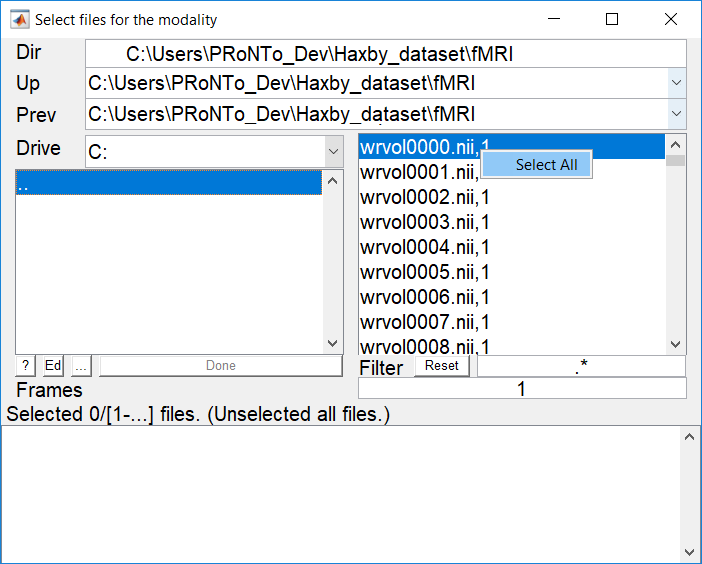
\includegraphics[scale=0.45]{images/Tutorial/v3/data_example1/gui_data_and_design_modality_files.png}
		  \captionsetup{width=0.9\linewidth}
	\captionof{figure}{`Files' field is used to select the scans/images for the selected subject.}
	\label{fig:gui_data_and_design_modality_files}
\end{minipage}%
	\begin{minipage}[b][7cm][b]{0.5\textwidth}
  \centering
		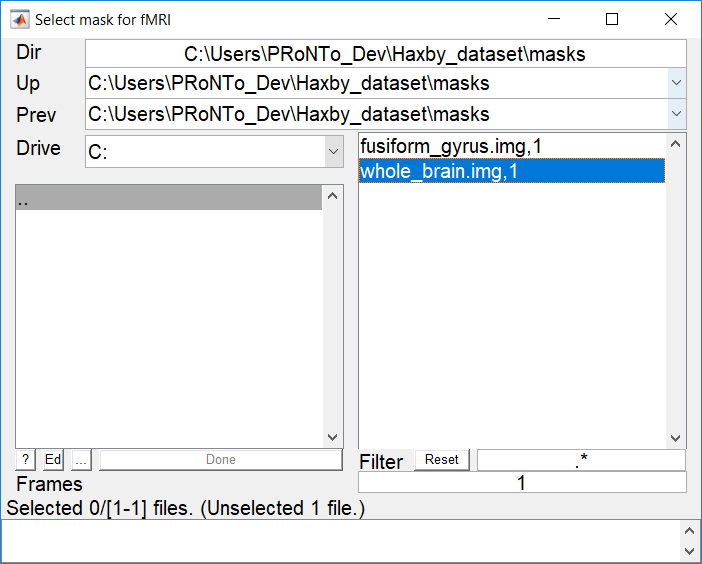
\includegraphics[scale=0.45]{images/Tutorial/v3/data_example1/gui_data_and_design_masks.png}
		\captionsetup{width=0.9\linewidth}
	\captionof{figure}{This window is called when one clicks `Masks'.}
	\label{fig:gui_data_and_design_masks}
	\end{minipage}
\end{figure}


	\item Click on `Review' button to check the data and the design inserted in this modality (Figure \ref{fig:gui_review_data}). For more information on what one can do with the Review option please see Chapter \ref{chap:DataDesign}.
	
	
\begin{figure}[!h]
	\centering
		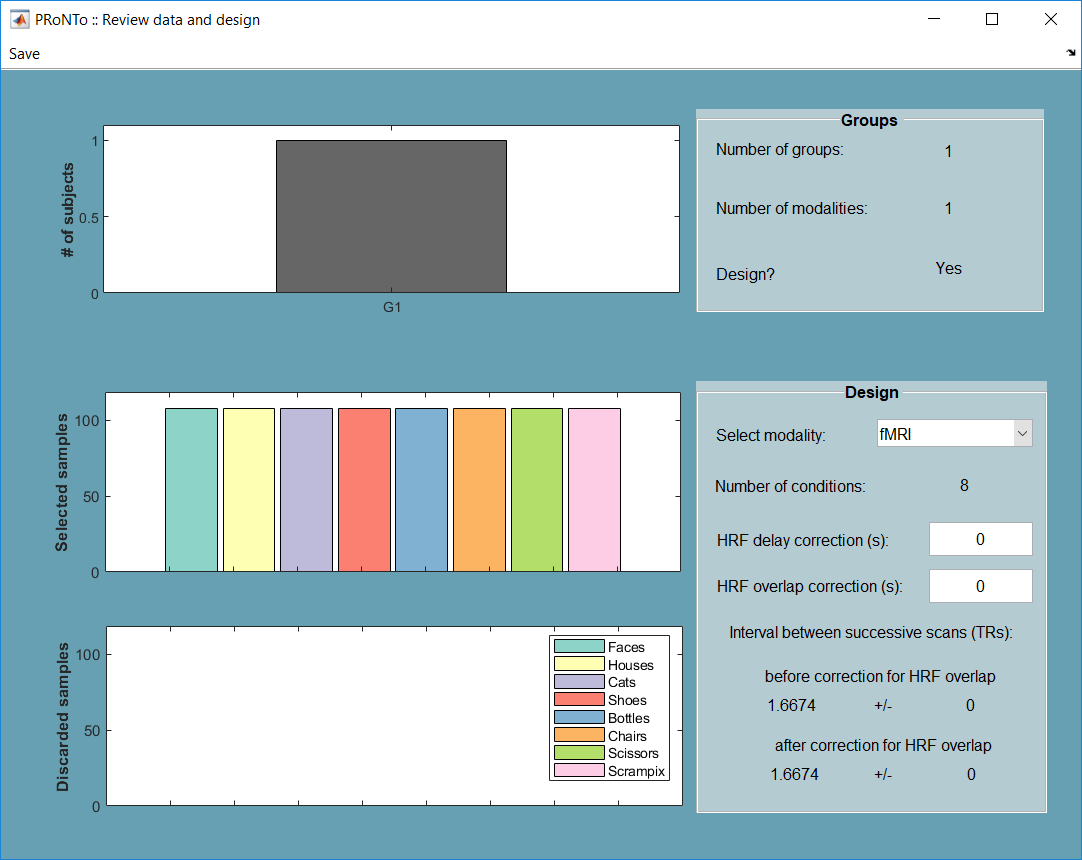
\includegraphics[scale=0.5]{images/Tutorial/v3/data_example1/gui_review_data.png}
	\caption{`Review' GUI allows the user to check the data and design.}
	\label{fig:gui_review_data}
\end{figure}	
	
	\item Click on `Save' button to create `PRT.mat' file with the structure containing the information that has been previously specified. If there is no error, the `Save' button changes color, from red to black; which also tells you that everything has been properly saved right up until that moment. The `Data and design' window after you click `Save' should look similar to the Figure \ref{fig:gui_data_and_designs_final}. If `Save' turned black and no errors are shown in the \matlab{} command window, leave the `Data and design' window by clicking `Quit'.
	

\begin{figure}[!h]
	\centering
		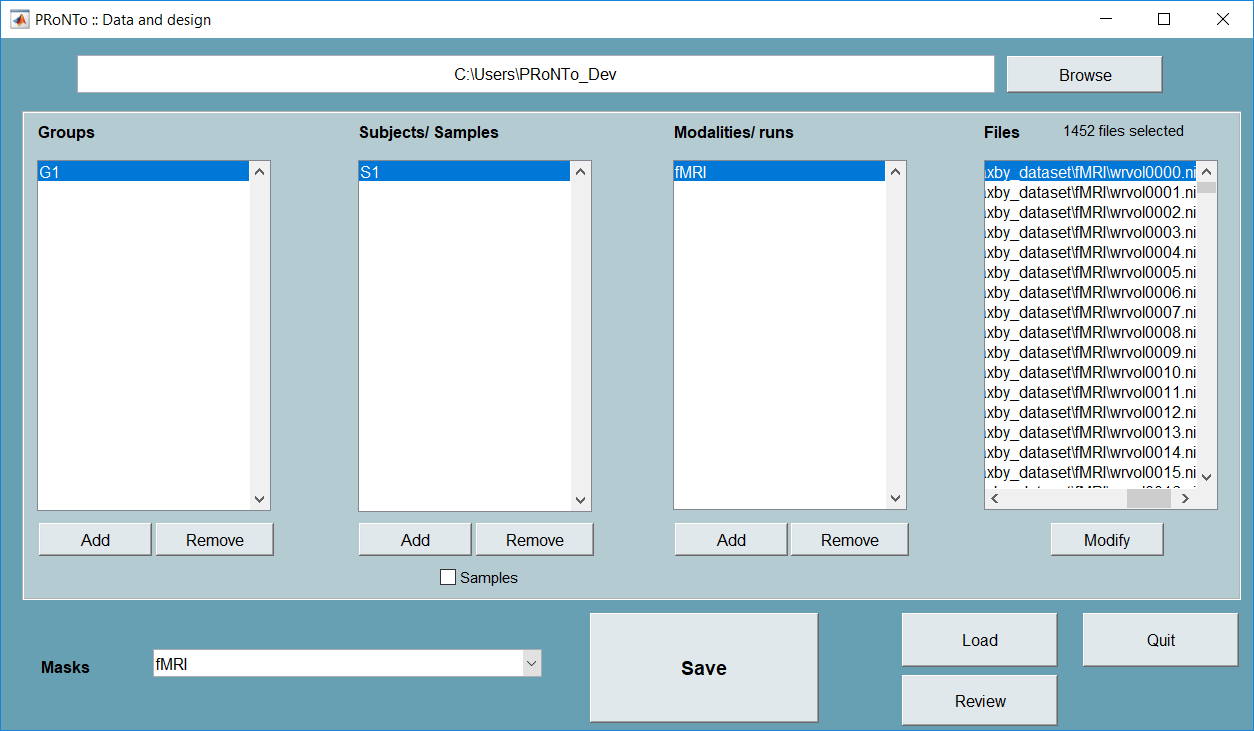
\includegraphics[scale=0.5]{images/Tutorial/v3/data_example1/gui_data_and_designs_final.png}
	\caption{`Data and design' GUI final configuration.}
	\label{fig:gui_data_and_designs_final}
\end{figure}	

\end{itemize}

%--------------------------------------------------------

\subsection{Prepare feature set}

\begin{itemize}
	
	\item Next we have to prepare the feature set, so click on `Prepare feature set' in PRoNTo's main window. A new window will open prompting you to select a PRT.mat file. Select the `PRT.mat' file previously created in the `Data \& Design' step (Figure \ref{fig:gui_prepare_featureSet_choose_PRT}).
	
	\begin{figure}[!h]
	    \centering
	    	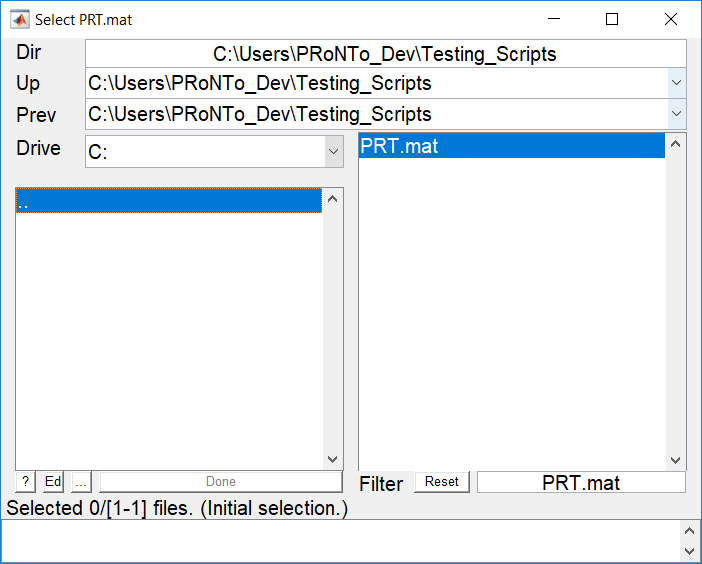
\includegraphics[scale=0.5]{images/Tutorial/v3/data_example1/gui_prepare_featureSet_choose_PRT.png}
    	\caption{`Prepare feature set' GUI.}
	    \label{fig:gui_prepare_featureSet_choose_PRT}
    \end{figure}
	
	\item Once you click `Done' another window will appear, `Specify modality to include' (Figure \ref{fig:gui_prepare_featureSet_specify_modality}). Here you set the specification of different parameters and options for each modality, which are: 
	
	\begin{itemize}
		\item `Modality' field: select the modality previously specified in the `Data \& Design' step, `fMRI'.
		\item `Conditions' field: select `All scans'.
		\item `Parameters box': select the polynomial detrend with order 1 and the 'No scaling' option.
		\item `Features box': leave the additional mask field as it is and the `build one kernel per region' tick box unchecked. Then, click on the `Done' button.  
		
			\begin{itemize}
			\item As an optional step, in the `Additional mask for selected modality' field, the user can specify a `second-level' mask, which can be used to select regions of interest (ROIs) on which the classification can be performed. For instance, we can enter the `fusiform\_gyrus' mask available with this dataset. 
			\end{itemize}
		
	\end{itemize}		
		
	\item Once you specify the modality to include and click `Done', yet another window will appear, `Prepare feature set'. Here you provide a name for the feature set, e.g. `HaxbyFeatures' and finally you click on `Build kernel / data matrix' to build the kernel. If everything was done correctly, a progress bar will pop up, marking the start of the procedure  (Figure \ref{fig:gui_prepare_featureSet_prepare_and_build}), which can take a few minutes.
	
% 			\begin{figure}[!h]
% 	\centering
% 		
\includegraphics[scale=0.55]{images/Tutorial/v3/data_example1/gui_prepare_featureSet_specify_modality.png}
% 	\caption{`Specify modality to include' GUI.}
% 	\label{fig:gui_prepare_featureSet_specify_modality}
% \end{figure}

% \begin{figure}[!h]
% 	\centering
% 		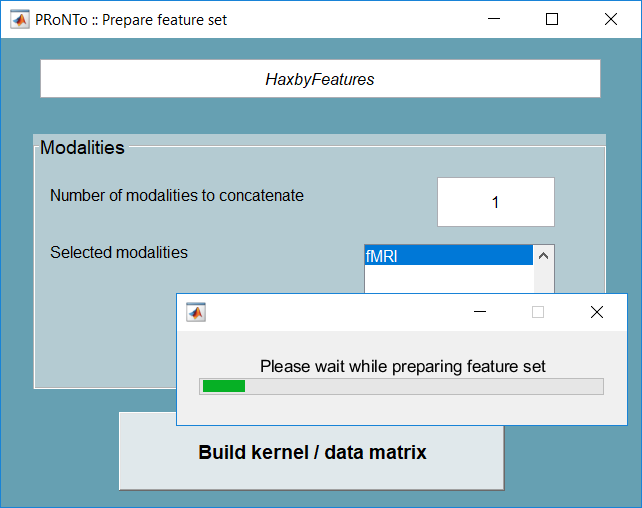
\includegraphics[scale=0.50]{images/Tutorial/v3/data_example1/gui_prepare_featureSet_prepare_and_build.png}
% 	\caption{Preparing feature set.}
% 	\label{fig:gui_prepare_featureSet_prepare_and_build}
% \end{figure}



\begin{figure}[!h]
	\centering
	\begin{minipage}[b][8.5cm][b]{0.5\textwidth}
  \centering
		
\includegraphics[scale=0.55]{images/Tutorial/v3/data_example1/gui_prepare_featureSet_specify_modality.png}
		  \captionsetup{width=0.9\linewidth}
	\captionof{figure}{`Specify modality to include' GUI.}
	\label{fig:gui_prepare_featureSet_specify_modality}
\end{minipage}%
	\begin{minipage}[b][8.5cm][b]{0.5\textwidth}
  \centering
	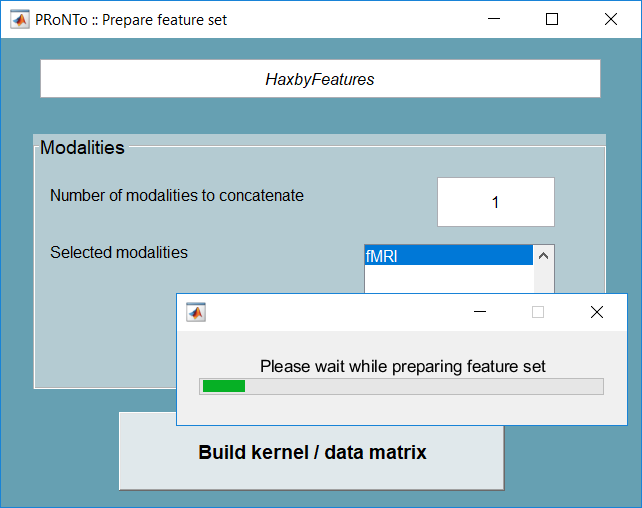
\includegraphics[scale=0.50]{images/Tutorial/v3/data_example1/gui_prepare_featureSet_prepare_and_build.png}
		\captionsetup{width=0.9\linewidth}
	\captionof{figure}{Preparing feature set.}
	\label{fig:gui_prepare_featureSet_prepare_and_build}
	\end{minipage}
\end{figure}

\end{itemize}


%---------------------------------------------------------------------

\subsection{Model: Specify new}

Next we have to specify a model. In PRoNTo's main window, click on `Specify new' and a new window will open, `Specify model' (Figure \ref{fig:gui_specify_new}).

\begin{itemize}
	
	\begin{figure}[!h]
	\centering
	\begin{minipage}[b][11.2cm][b]{0.5\textwidth}
  \centering
		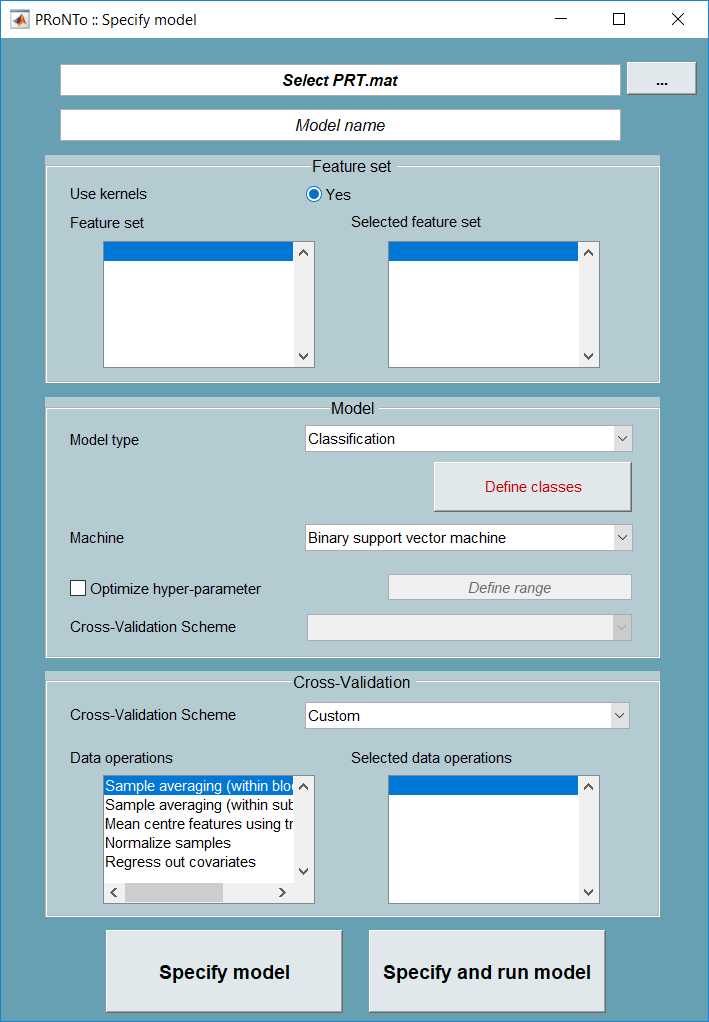
\includegraphics[scale=0.5]{images/Tutorial/v3/data_example1/gui_specify_new.png}
		  \captionsetup{width=0.9\linewidth}
	\captionof{figure}{`Model: Specify new' GUI.}
    	\label{fig:gui_specify_new}
\end{minipage}%
	\begin{minipage}[b][11.2cm][b]{0.5\textwidth}
  \centering
	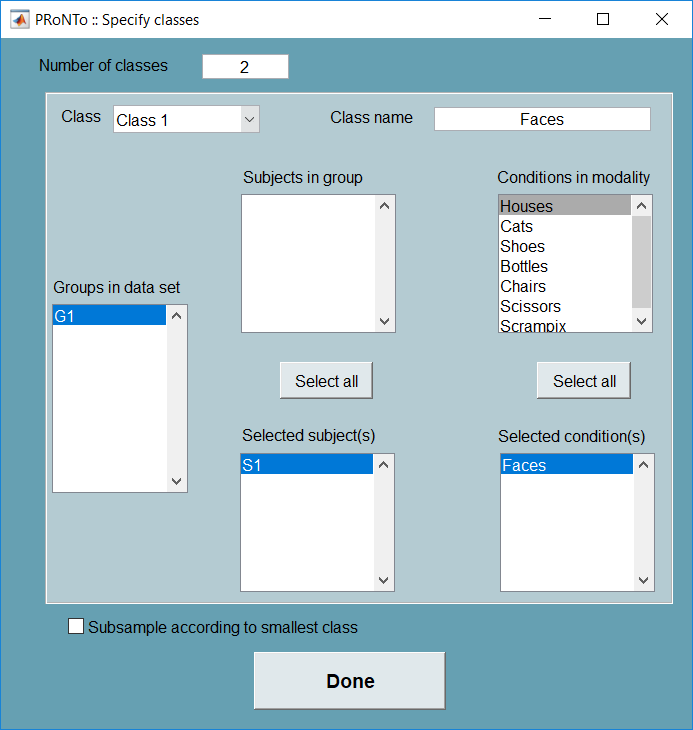
\includegraphics[scale=0.6]{images/Tutorial/v3/data_example1/gui_specify_new_specify_classes.png}
		\captionsetup{width=0.9\linewidth}
	\captionof{figure}{`Specify classes' GUI.}
    	\label{fig:gui_specify_new_specify_classes}
	\end{minipage}
\end{figure}
	
    \begin{figure}[h!]
    	\centering
	    	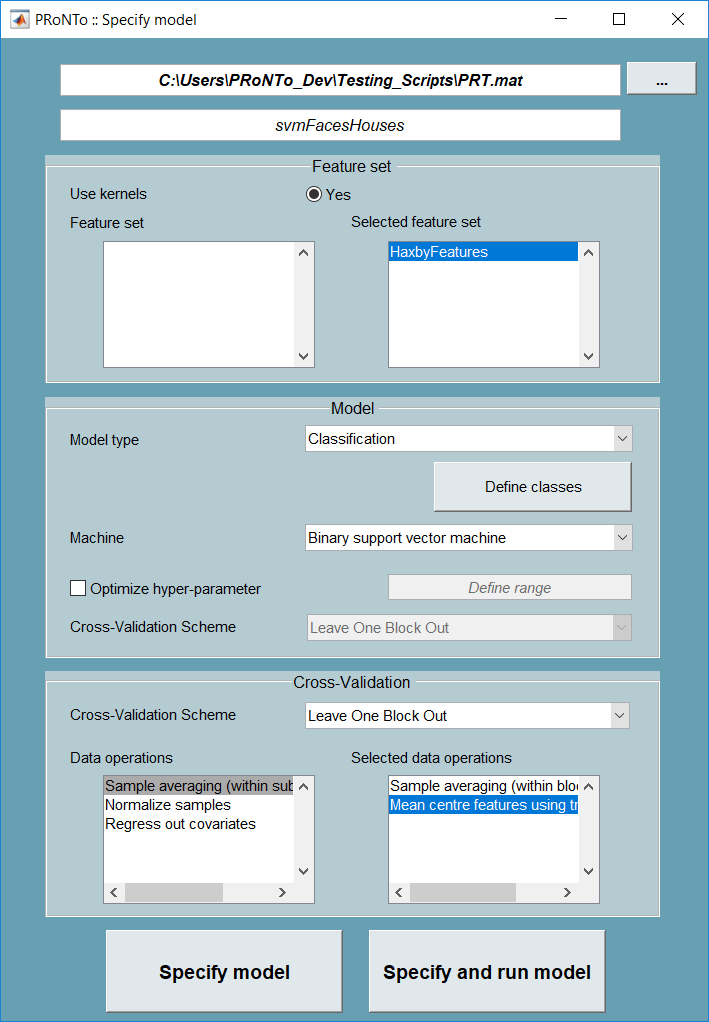
\includegraphics[scale=0.5]{images/Tutorial/v3/data_example1/gui_specify_new_final_config.png}
	    \caption{`Model: Specify new' GUI final configuration.}
	    \label{fig:gui_specify_new_final_config}
    \end{figure}
    
	
	\item Select the `PRT.mat' file and provide a name to the model, e.g. `svmFacesHouses'.

	\item Select from the list one of the `Feature Set' previously defined. In this case, there is only one `HaxbyFeatures', but in general from v3.0 you are free to choose more than one feature set that can be combined using Multiple Kernel Learning.

	\item	Leave the option `Use kernels' tick box as it is, i.e. `Yes'.

	\item	Select the `Classification' model type and click on `Define classes' button. A new window will open, `Specify classes' (Figure \ref{fig:gui_specify_new_specify_classes}), to define the number of classes and a name for each class. We will define 2 classes. First click `Class 1' on the tab `Class'. For `Class 1' select subject `S1' and the condition `Faces' and, similarly, for `Class 2' select subject `S1' and the condition `Houses'. Leave the `Subsample according to smallest class' as it is for now. Once you have appropriately specified everything, click `Done'.
	
	\item Select the `Binary support vector machine' option, in the `Machine' field.
	
	\item Leave the option `Optimize hyper-parameter' tick box unchecked and `Cross-Validation Scheme' (internal loop) as it is. 
	
	\item Select the `Leave One Block Out' cross-validation scheme (external loop).
	
	\item In the `Data operations' box, select the `Sample averaging (within block)' option, which corresponds to a temporal compression of the data within each block, and `Mean centre features using training data' option. Then, the `Specify model' window should look similar to Figure \ref{fig:gui_specify_new_final_config}.
	
	\item Click on `Specify and run model' and the model will be immediately estimated, therefore there is no need to use the `Run model' module in this case. However if you wish to run permutation tests you need to specify this in the `Run model' module.

	\item If you do not wish to average the scans within each block (i.e. to do temporal compression), go back to the `Specify model' window, give another name to the model and select the same options mentioned above, except in the data operations part. Here, choose only the `Mean centre features using training data' option. Finish by clicking on the `Specify and run model' button.

\end{itemize}

%--------------------------------------------------------------------

\subsection{Model: Specify from (optional step)}
\label{gui_specify_model_from}

\begin{itemize}
    
    \item The `Specify from' window is the same as the `Specify new' window, except that some fields have been disabled to ensure comparability of the models, and there is also an extra popup menu that allows to select which model to copy from (Figure \ref{fig:gui_specify_from}). For more information on what one can do with the `Specify from' option please see Chapter \ref{chap:ModelCrossV}.
    
    \item Select the `PRT.mat' file we have been using so far and provide a new name for the model. It's recommended giving a meaningful name to the model so that there is no confusion later on. We previously used SVMs, so now we can try a different machine for comparison, for example the Gaussian Process (GP) classifier, so we can name it  `gpFacesHouses'. Alternatively, assuming you had previously created a second feature set called `HaxbyFeatures2' or another more meaningful name according to your preference, you could now try also deselecting `HaxbyFeatures' and selecting for example `HaxbyFeatures2' as your selected feature set.

    \item  Notice that Classes/Regression selection and outer CV options cannot be modified. Only the `Machine' (with its hyper-parameter optimization), the feature sets and the `Data operations' can be modified when using specifications from a previously defined model.
    
    \item  After you have specified everything, the final configuration would look like the one in Figure \ref{fig:gui_specify_from_final_config}. Now click `Specify and run model' to create a second model comparable to `svmFacesHouses' model.

	\begin{figure}[!h]
	\centering
	\begin{minipage}[b][11.5cm][b]{0.5\textwidth}
  \centering
		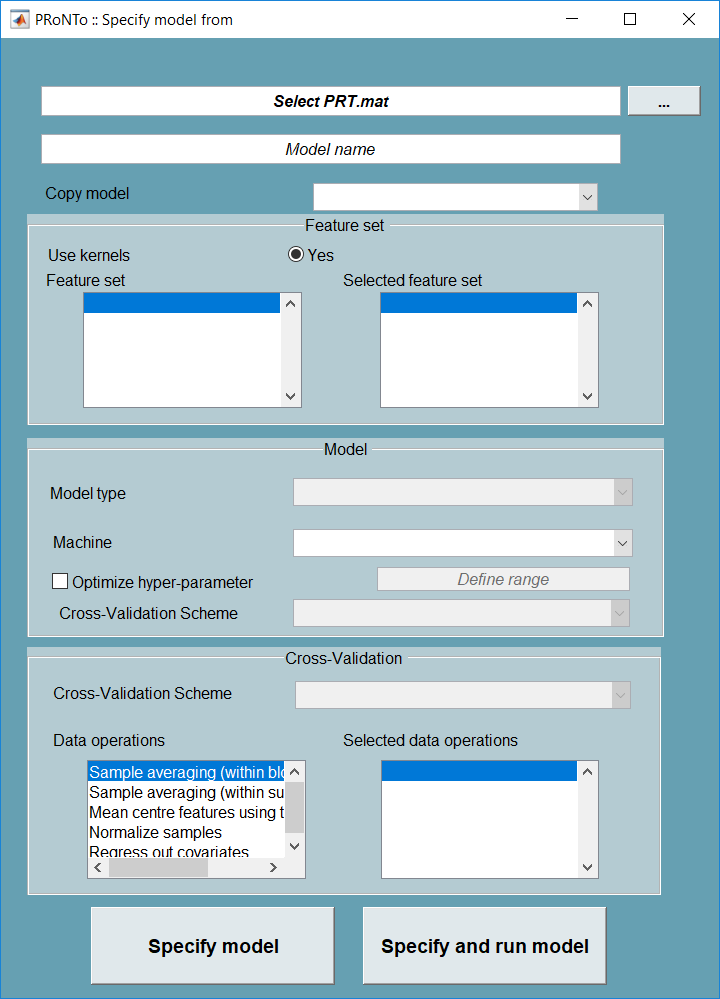
\includegraphics[scale=0.5]{images/Tutorial/v3/data_example1/gui_specify_from.png}
		  \captionsetup{width=0.9\linewidth}
	\captionof{figure}{`Model: Specify from' GUI.}
	        \label{fig:gui_specify_from}
\end{minipage}%
	\begin{minipage}[b][11.5cm][b]{0.5\textwidth}
  \centering
	
\includegraphics[scale=0.5]{images/Tutorial/v3/data_example1/gui_specify_from_final_config.png}
		\captionsetup{width=1.1\linewidth}
	\captionof{figure}{`Model: Specify from' GUI final configuration.}
	        \label{fig:gui_specify_from_final_config}
	\end{minipage}
\end{figure}

\end{itemize}

For further information the reader should look at the tutorial of Chapter \ref{chap:ModelCrossV}.


%--------------------------------------------------------------------

\subsection{Model: Run}
\label{run_model}
\begin{itemize}
    
    \item From the `Run model' window you can run the model(s) you have specified in the previous section. It is useful when you have specified some model(s) but did not run it/them, and also if you want to run permutations for multiple models (Figure \ref{fig:gui_run}).

        \begin{figure}[h!]
        	\centering
	        	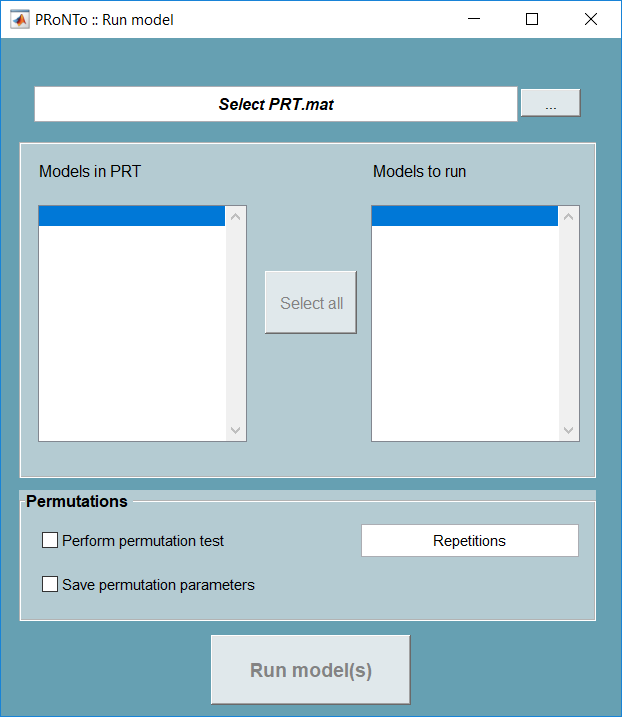
\includegraphics[scale=0.5]{images/Tutorial/v3/data_example1/gui_run.png}
        	\caption{`Model: Run' GUI.}
	        \label{fig:gui_run}
         \end{figure}
         
     \item If you want to run permutation tests, check the options `Perform permutation test' and `Save permutation parameters', and also specify the number of repetitions. Keep in mind that in order to check the significance of the results you must run permutation tests. It has been shown that 1000 repetitions approximate well the null distribution, so it's best if you are as close to that number as possible.

\end{itemize}
  
%--------------------------------------------------------------------

\subsection{Display model (optional step)}

\begin{itemize}
\item To review the model specification, in the main PRoNTo GUI, click on `Review kernel \& CV' and after you select the `PRT.mat' file to review, a new window will open, `Review Model Specification' (Figure \ref{fig:gui_review_kernel_and_CV}).

\begin{figure}[h!]
	\centering
		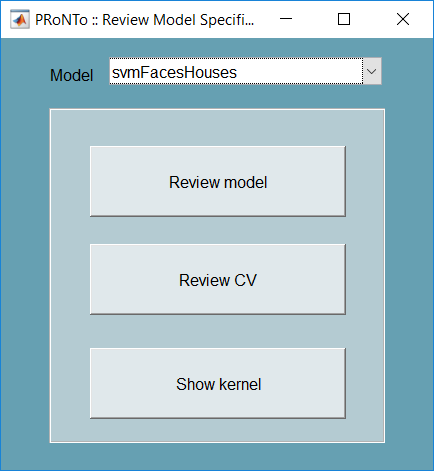
\includegraphics[scale=0.5]{images/Tutorial/v3/data_example1/gui_review_kernel_and_CV.png}
	\caption{Review CV \& kernel window.}
	\label{fig:gui_review_kernel_and_CV}
\end{figure}

\item Select the model, `svmFacesHouses', from the list at the top and click on `Review model'; then, select one class from the list of `Class' to see which groups, subjects and conditions this class comprises (Figure \ref{fig:gui_review_kernel_and_CV_model}).

\begin{figure}[h!]
	\centering
		
\includegraphics[scale=0.5]{images/Tutorial/v3/data_example1/gui_review_kernel_and_CV_model.png}
	\caption{Review model specification window for Class 1.}
	\label{fig:gui_review_kernel_and_CV_model}
\end{figure}

\item To review the data and cross-validation matrix click on `Review CV' (Figure \ref{fig:gui_review_kernel_and_CV_CV}). For more information on what these matrices mean, please consult chapter \ref{chap:ModelCrossV}.

\begin{figure}[h!]
	\centering
		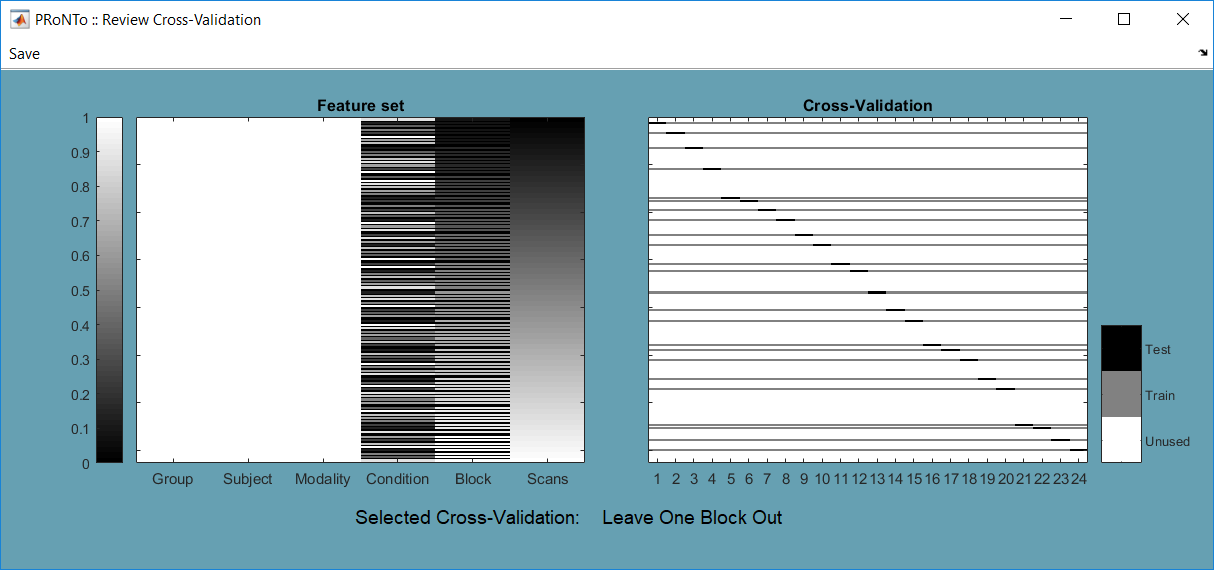
\includegraphics[scale=0.5]{images/Tutorial/v3/data_example1/gui_review_kernel_and_CV_CV.png}
	\caption{Data and cross-validation matrix from `Review CV' option.}
	\label{fig:gui_review_kernel_and_CV_CV}
\end{figure}


\item To review the kernel, click on `Show kernel' (Figure \ref{fig:gui_review_kernel_and_CV_kernel}).

\end{itemize}

	\begin{figure}[!h]
	\centering
	\begin{minipage}[b][8.5cm][b]{0.5\textwidth}
  \centering
		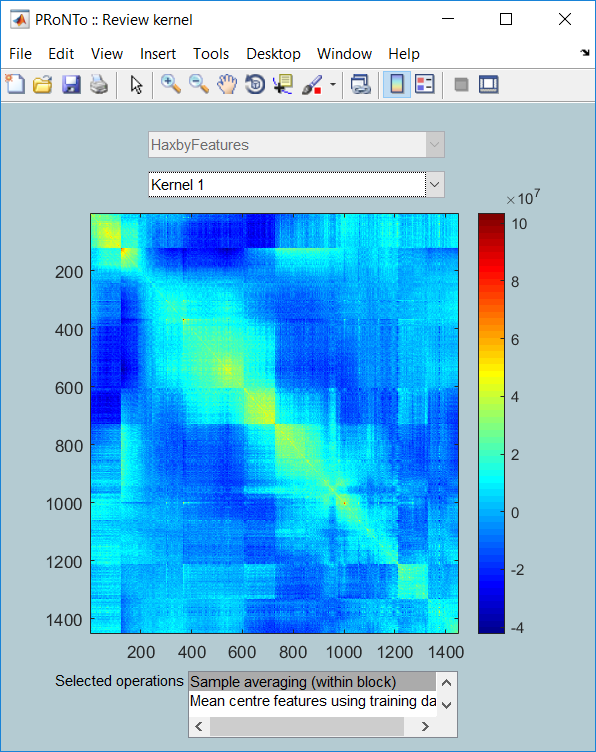
\includegraphics[scale=0.5]{images/Tutorial/v3/data_example1/gui_review_kernel_and_CV_kernel.png}
		  \captionsetup{width=0.9\linewidth}
	\captionof{figure}{Kernel matrix used for classification.}
	\label{fig:gui_review_kernel_and_CV_kernel}
\end{minipage}%
	\begin{minipage}[b][8.5cm][b]{0.5\textwidth}
  \centering
	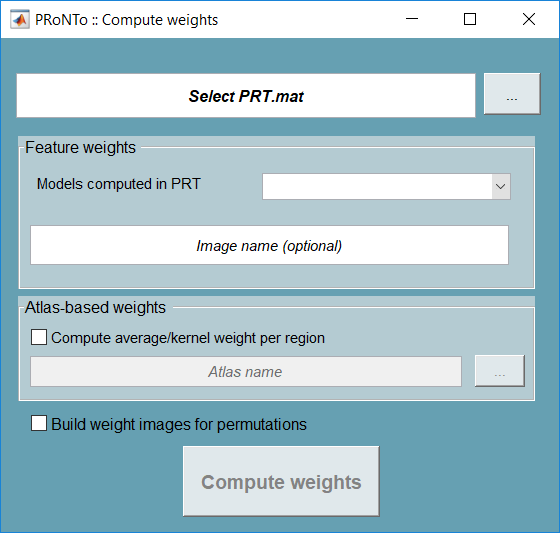
\includegraphics[scale=0.5]{images/Tutorial/v3/data_example1/gui_compute_weights.png}
		\captionsetup{width=1\linewidth}
	\captionof{figure}{`Compute weights' GUI.}
	\label{fig:gui_compute_weights}
	\end{minipage}
\end{figure}

%----------------------------------------------------

\subsection{Display results}
\label{display_results}

\begin{itemize}
	
	\item In PRoNTo's main window, click on `Display results' and select the `PRT.mat' file. This will open the main results window. In the `Model' panel, select the model that you want to view, `svmFacesHouses'. The main results window together with the performance stats should be similar to the one in Figure \ref{fig:gui_display_results}.
	
\begin{figure}[h!]
	\centering
		
\includegraphics[scale=0.5]{images/Tutorial/v3/data_example1/gui_display_results.png}
	\caption{`Results' GUI.}
	\label{fig:gui_display_results}
\end{figure}
	
	\item In the `Results' window, one can select specific folds in the `Fold' list and also check their performance with different plots in the `Plot' list.
	
	\item Keep in mind that if you have not run permutation tests, the values of `BA p-value' and `CA p-value' would be `N.A.'.

\end{itemize}

A very important change in v3 is that model performance is computed within folds, and then the stats are averaged across all folds. In v2, stats were computed within folds but then predictions were concatenated across folds to produce the model-level stats. This has been advised against as being over-optimistic. For further information regarding that the reader is referred to chapter \ref{chap:ModelCrossV}. This change is reflected in the `Display results' window: the list of plots available across folds is not the same as the list of plots available within folds.
\\[1cm]

\noindent Across fold the user can display:

\begin{itemize}
    \item `Accuracy distribution': The balanced accuracy in each fold plotted as a violin plot, with its mean displayed in red. If permutations were estimated, the left side of the violin corresponds to the accuracy distribution (with additional histogram), while the right side corresponds to the distribution of average balanced accuracy with permuted labels.

    \item `Predictions': Same as v2.

    \item `ROC': In v2, the ROC was built from the concatenated function values. In v3, we now build the average ROC curve and display its standard deviation across folds as shaded area.

    \item `Influence of the hyper-parameters': Similar to v2, but added scatter plot representing the balanced accuracy within each fold for each value of the hyper-parameter.

\end{itemize}

\noindent Within folds, the plots are the same as in v2. Minor changes were performed to improve their appearance.
	
%------------------------------------------------------------------

\subsection{Compute weights (optional step)}

\begin{itemize}
\item In PRoNTo's main window, click on `Compute weights' and a new window will open, `Compute weights' (Figure \ref{fig:gui_compute_weights}).

\item Select the `PRT.mat' file.

\item Select the model from the list of `Models computed in PRT', `svmFacesHouses' model.

\item If you previously run permutation tests and want to review and display the weights for the permutations, check the option `Build weight images for permutations'. Note that this option will create one weight image for each permutation.

\item Leave the option `Compute average/kernel weight per region' unchecked.

\item Click on `Compute weights' button. Computations will be displayed on the \matlab{} command window.

\end{itemize}

%------------------------------------------------------------------

\subsection{Display weights}

\begin{itemize}
	
	\item In PRoNTo's main window, click on `Display weights' and select the `PRT.mat' file. This will open the `Model interpretation' window.
	
	\item By clicking on `Model', svmFacesHouses, an image will appear in the `Weights map' box. To show the `Anatomical img' you have to load an anatomical image for reference. A template image can be found in SPM's canonical folder (`single\_subj\_T1` file). The final window will look similar to the one shown in Figure \ref{fig:gui_display_weights_final}.

\begin{figure}[h!]
	\centering
		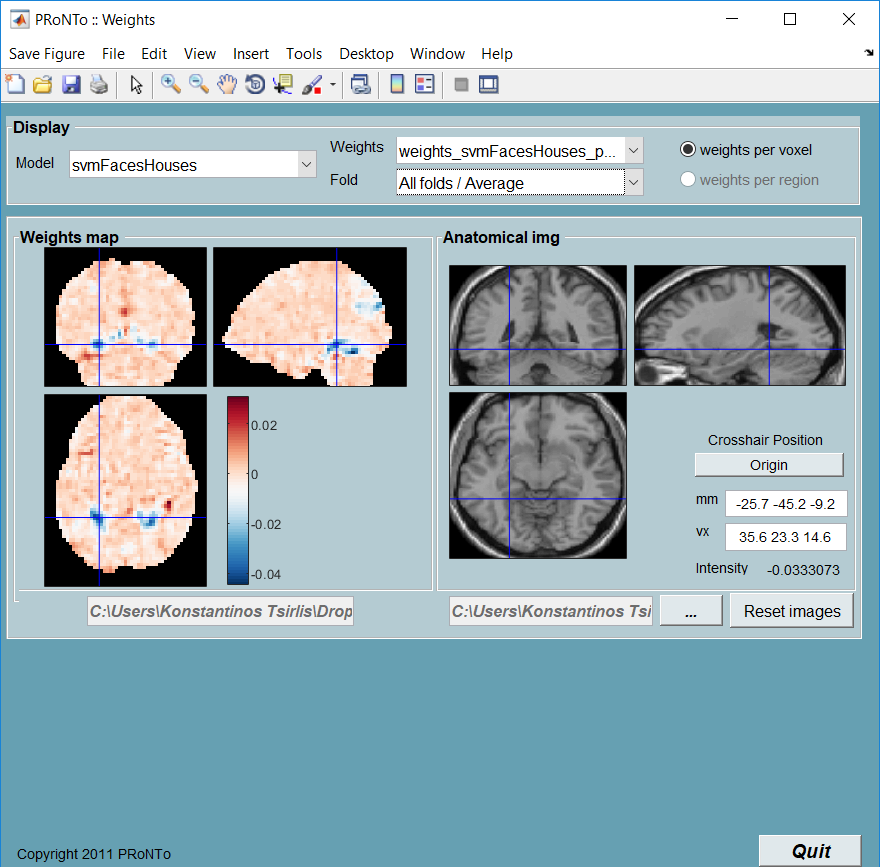
\includegraphics[scale=0.5]{images/Tutorial/v3/data_example1/gui_display_weights_final.png}
	\caption{`Model interpretation' GUI with results.}
	\label{fig:gui_display_weights_final}
\end{figure}
	
\end{itemize}

%=====================================================



%=====================================================

\section{Batch analysis}
\label{sec:Batch_analysis_svm}

This tutorial will now show how to analyse the same data but using the {\tt matlabbatch} system. \\

Once again, create a new directory where you wish to save the results. On the main interface of PRoNTo click on the `Batch' button to open the `{\tt matlabbatch}'. Alternatively, type `prt\_batch' on the \matlab{} command window. On the menu bar of the batch, there is a PRoNTo menu with the 6 options shown in the main steps interface (Figure \ref{fig:batch_main}).

%--------------------------------------------------------------

\subsection{Data \& Design}
\label{batch_data_and_design}

\begin{itemize}

	\item Click on `Data \& Design' in the PRoNTo menu. Figure \ref{fig:batch_data_and_design} is the starting `Data \& Design' module menu and Figure \ref{fig:batch_data_and_design_full} is the full drop-down list of options. All modules follow the same general structure with some initial options appearing at first, that have a variety of sub-options that appear once you specify them. Figure \ref{fig:batch_data_and_design_full_final} is the final configuration of the {\tt matlabbatch} `Data \& design' module.
	
	\begin{figure}[!h]
	\centering
	\begin{minipage}[b][8.5cm][b]{0.5\textwidth}
  \centering
		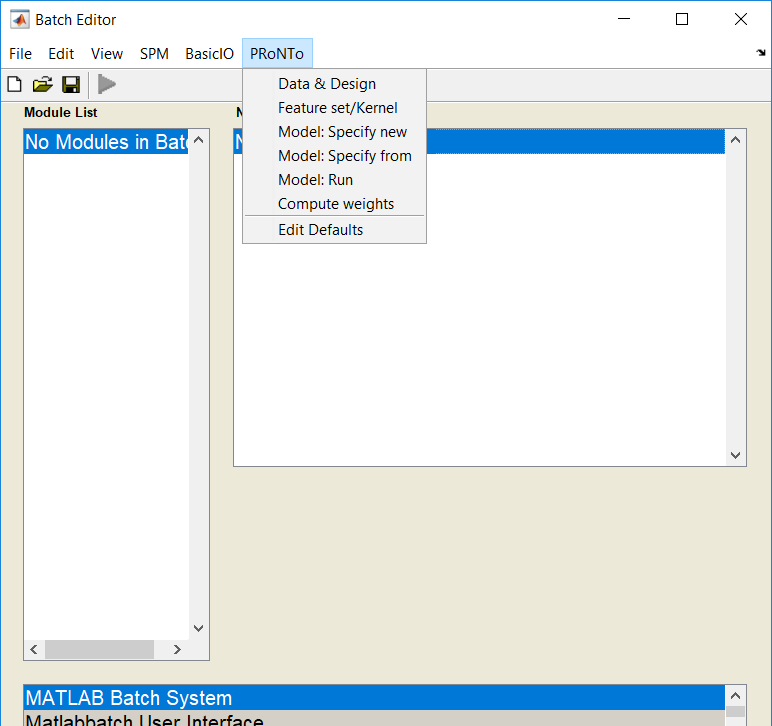
\includegraphics[scale=0.5]{images/Tutorial/v3/data_example1/batch_main.png}
		  \captionsetup{width=0.9\linewidth}
	\captionof{figure}{Menu PRoNTo in the main {\tt matlabbatch} window.}
	\label{fig:batch_main}
\end{minipage}%
	\begin{minipage}[b][8.5cm][b]{0.5\textwidth}
  \centering
	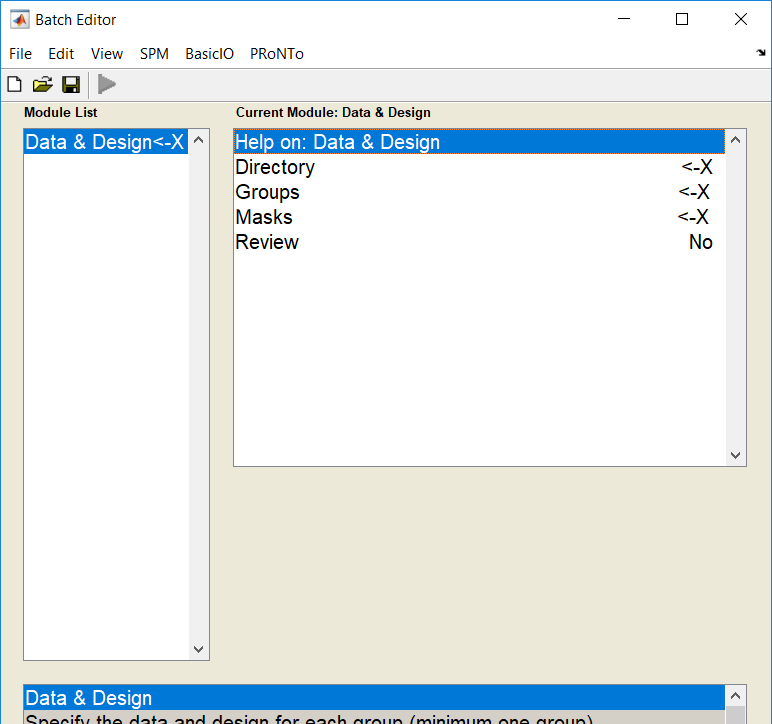
\includegraphics[scale=0.5]{images/Tutorial/v3/data_example1/batch_data_and_design.png}
		\captionsetup{width=1\linewidth}
	\captionof{figure}{`Data \& design' module in {\tt matlabbatch} window. }
    	\label{fig:batch_data_and_design}
	\end{minipage}
\end{figure}
	
	\begin{figure}[!h]
	\centering
	\begin{minipage}[b][8cm][b]{0.5\textwidth}
  \centering
		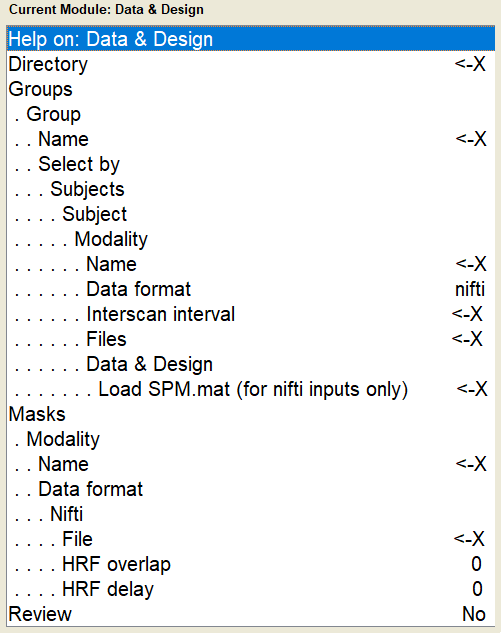
\includegraphics[scale=0.5]{images/Tutorial/v3/data_example1/batch_data_and_design_full.png}
		  \captionsetup{width=0.9\linewidth}
	\captionof{figure}{Drop-down list of options in the {\tt matlabbatch} `Data \& design' module.}
    	\label{fig:batch_data_and_design_full}
\end{minipage}%
	\begin{minipage}[b][8cm][b]{0.5\textwidth}
  \centering
	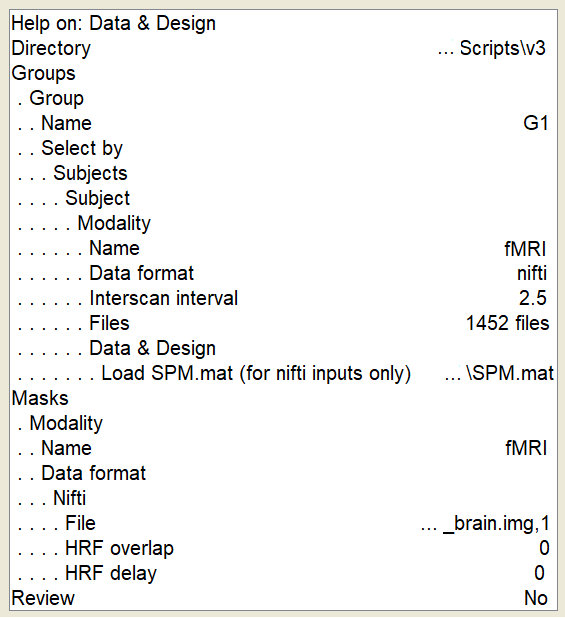
\includegraphics[scale=0.5]{images/Tutorial/v3/data_example1/batch_data_and_design_full_final.png}
		\captionsetup{width=1\linewidth}
	\captionof{figure}{Final configuration of the {\tt matlabbatch} `Data \& design' module.}
    	\label{fig:batch_data_and_design_full_final}
	\end{minipage}
\end{figure}

	\item In the `Directory' field, select a directory where the `PRT.mat' file will be saved. There are three ways of editing all fields in {\tt matlabbatch}: (i) by using the right mouse button and clicking on the current option, (ii) clicking on current button in the window or (iii) by double clicking.
	
	\item In the `Groups' field:
 	
		\begin{itemize}
		
		\item Add one group.
		
		\item In the field `Name', provide a name without spaces to that group, e.g. `G1'. 
		
		\item In the field `Select by', select the `Subjects' option and add one subject.
		
		\item Add one modality for this subject and provide a name, e.g. `fMRI'; choose the appropriate data format (here nifti); define the interscan interval of 2.5 seconds; and in the field `Files', select all the image files available in the fMRI directory of the Haxby dataset.	
		
		\item In the `Data \& Design' field, since our data are in nifti format, choose the `Load SPM.mat' option. This file is available with the Haxby dataset on PRoNTo's website\footnote{http://www.mlnl.cs.ucl.ac.uk/pronto/prtdata.html} inside the folder Haxby\_dataset/design/.
% 		The batch editor should look similar to the one in Figure \ref{fig:batchGroups}.

        \item In case our data were in MEEG format, we could choose the `Events in MEEG file' option, where we could also further specify regression targets/covariates.
		
% 		\begin{figure}[h!]
% 	\centering
% 		
\includegraphics[scale=0.6]{images/Tutorial/batchGroups.png}
% 	\caption{Data and design module in {\tt matlabbatch}. }
% 	\label{fig:batchGroups}
% 	\end{figure}
				
		
		\begin{itemize}
	
			\item In case there is no `SPM.mat' or `MEEG Events' file available to use, create a new design by selecting the option `Specify design'. Choose the units (scans in our case), how many conditions you have, which in this case are 8 conditions (corresponding to the 8 categories of images) and also write the names, onsets, durations and any covariates and/or regression targets of each condition (Figure \ref{fig:batch_data_and_design_specify_design}). For further information on how to enter covariates and/or regression targets the reader should look at the tutorial of Chapter \ref{data_example2}.
	
\begin{figure}[h!]
	\centering
		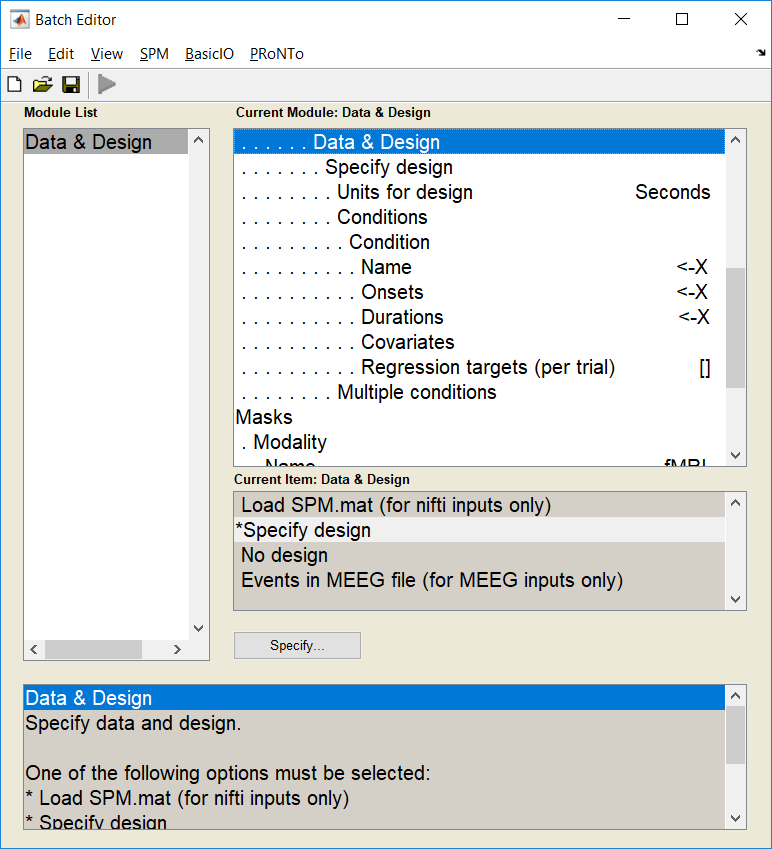
\includegraphics[scale=0.5]{images/Tutorial/v3/data_example1/batch_data_and_design_specify_design.png}
	\caption{`Data \& design' module. The `Specify design' option.}
	\label{fig:batch_data_and_design_specify_design}
\end{figure}
	
	\end{itemize}

		\end{itemize}
	
	\item In the `Masks' field, add a new modality and provide the same modality name, `fMRI', choose the appropriate data format and finally select the `whole\_brain' mask available in the masks directory of the Haxby dataset. The name of the modality here has to be exactly the same as in `Modalities', otherwise it will not work.
	
	%checar aqui
	
	\item Leave the `HRF overlap' and the `HRF delay' fields as default.
	
	\item In the `Review' field, select `Yes' if you would like to review your data and design in a separate window. Otherwise, leave as it is, i.e. `No'. Keep in mind that the procedure pauses while you review the data and that you have to close the `Review' window for the procedure to continue.


\end{itemize}

%------------------------------------------------------------

\subsection{Feature set / Kernel}

\begin{itemize}
	\item Click on `Feature set / Kernel' option on PRoNTo's {\tt matlabbatch} menu.
	
	\item With `Load PRT.mat' field selected, click on the `Dependency' button to associate the `PRT.mat' file created in the previous `Data \& Design' step or click on the `Select files' button to browse where `PRT.mat' file was saved. The window of Figure \ref{fig:batch_feature_set_dep} is called to establish a dependency connection with the previous `Data \& design' module.
	
\begin{figure}[!h]
	\centering
	\begin{minipage}[b][10cm][b]{0.5\textwidth}
  \centering
		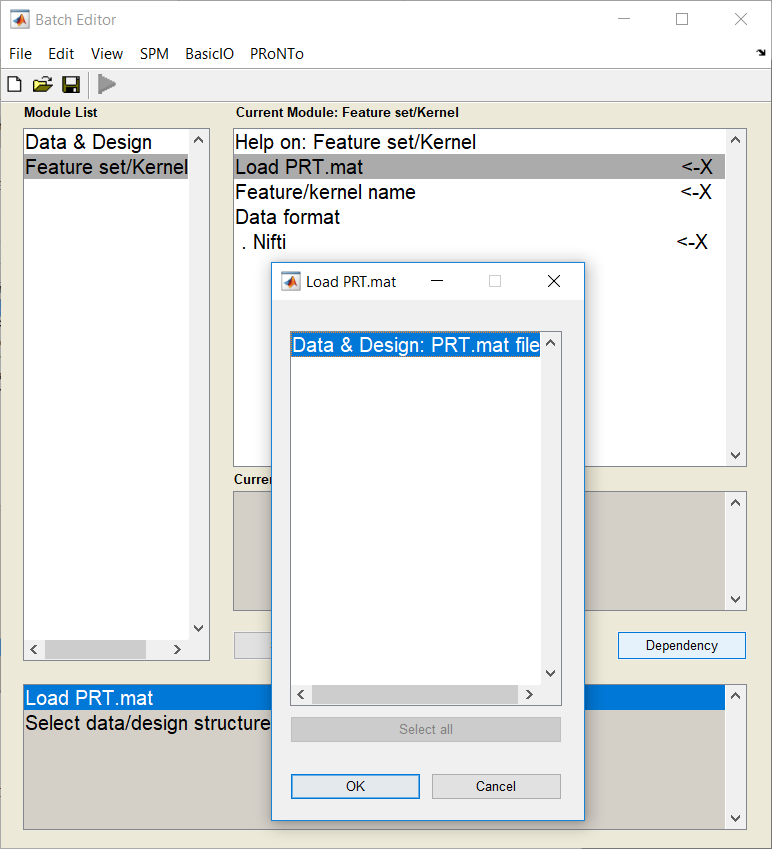
\includegraphics[scale=0.5]{images/Tutorial/v3/data_example1/batch_feature_set_dep.png}
		  \captionsetup{width=0.9\linewidth}
	\captionof{figure}{`Feature set / Kernel' module in {\tt matlabbatch}.}
	\label{fig:batch_feature_set_dep}
\end{minipage}%
	\begin{minipage}[b][10cm][b]{0.5\textwidth}
  \centering
	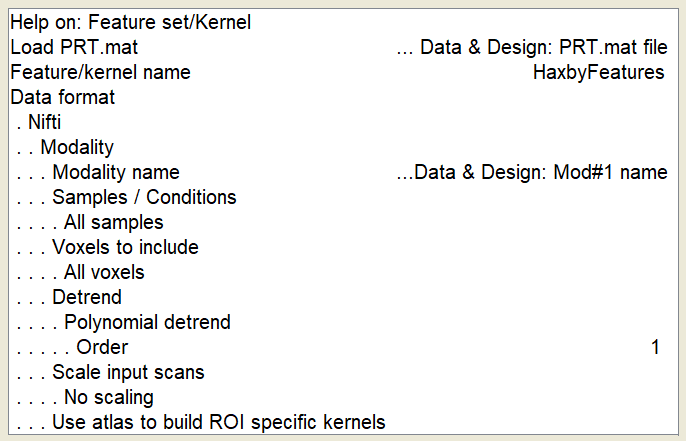
\includegraphics[scale=0.5]{images/Tutorial/v3/data_example1/batch_feature_set_full_final.png}
		\captionsetup{width=1\linewidth}
	\captionof{figure}{Final configuration of the {\tt matlabbatch} `Feature set / Kernel' module.}
	\label{fig:batch_feature_set_full_final}
	\end{minipage}
\end{figure}


	\item Provide a name to the `Feature/kernel' set, e.g. `HaxbyFeatures'.
	
	\item Select the `nifti' option for a data format, add one modality and select the modality name with the `Dependency' button\footnote{Or type it in manually, `fMRI', but the name needs to be {\it exactly} the same as the one specified in the `Data \& Design' module.}(Data \& Design:Mod\#1 name).
	
		\begin{itemize}
	
	\item In the `Samples/Conditions' field , select the `All samples' option.
	
	\item In the `Voxels to include' field, select `All voxels' option, this means we are not entering an additional second-level mask.
	
			\begin{itemize}
			\item This is an optional step. In the `Voxels to include' options, the user can specify a `second-level' mask, which would define regions of interest (ROIs) on which the classification can be performed. In this case, select the `fusiform\_gyrus' mask.
			\end{itemize}
	
	\item In the `Detrend' field, select `Polynomial detrend' option with order 1.
	
	\item In the `Scale input scans' field, select `No scaling' option and finally leave `Use atlas to build ROI specific kernels' as default.
	
	\end{itemize}
	
	\item Figure \ref{fig:batch_feature_set_full_final} is the final configuration of the {\tt matlabbatch} `Feature set / Kernel' module. For the other Data formats please refer to Chapter \ref{sec:multimodal_face}.

\end{itemize}

%--------------------------------------------------------

\subsection{Model: Specify new}

\begin{itemize}

\item Click on `Model: Specify new' option on PRoNTo's {\tt matlabbatch} menu.
	
	\item With `Load PRT.mat' field selected, click on `Dependency' button to associate the `PRT.mat' file created in the previous `Feature set / Kernel' step, or alternatively either double-click on `Load PRT.mat' option or click on `Specify' button to browse where `PRT.mat' file was saved.

	\item Provide a name to the model, e.g. `svmFacesHouses'. 
	
	\item In the `Feature sets' field, select the feature set name with the `Dependency' button\footnote{or write it {\it exactly} as previously defined in the `Feature set / Kernel' module (option `Feature set/Kernel: Feature/kernel name'), here `HaxbyFeatures'.}.
	
	\item Select the `Classification' model type:
	
		\begin{itemize}
		
		\item Add 2 new classes.
		
		\item For Class (1) write `Faces' on the name field and add one group. Select the group name from the `Data \& Design' module (`Data \& Design:Group\#1 name') with the `Dependency' button\footnote{Or write it {\it exactly}, as previously defined in the Data \& Design' module, here `G1'}. Similarly, for Class (2) write `Houses' on the name field and add the group created in the `Data \& Design' module, `G1'.	
		
		\item In the `Subjects' field, type `1' (only subject 1 is selected).
		
		\item In the `Conditions / Scans' field, select the `Specify Conditions' option and add a new condition. Provide a name for this condition, i.e. for Class (1) `Faces' and for Class (2) `Houses'. Note that this name needs to be spelled exactly as specified in the `Data \& Design' module: if you simply loaded an `SPM.mat' file for the design, you {\it must} know the names of the conditions.
		

		\end{itemize}			
	
        \item Leave `Subsample examples based on class definition' as it is, i.e. `No'.
		
	\item In the `Machine Type' field:

	\begin{itemize}
	
	\item Select the `Kernel machine' and the `SVM Classification' options.

    \item Leave the `SVM string argument' as it is, i.e. `-q -s 0 -t 4 -c'.	
    
	\item Finally, on the `Machine optimization and parameters' field select `No optimization'.
	
	\end{itemize}
	
	\item In the `Cross-validation type' field, select `Leave one block out' option.
	
	\item Leave the `Include all scans' field as it is, i.e. `No'.

	\item In the `Data operations' field:
	
		\begin{itemize}
		\item  Leave the `Mean centre features' field as it is, i.e. `Yes'. 
				
		\item  Leave the `Other Operations' field as it is, i.e. `No operations'.
		\end{itemize}
	
\end{itemize}

Figure \ref{fig:batch_model_specify_new_full_final} is the final configuration of the {\tt matlabbatch} `Model: Specify new' module.

\begin{figure}[!h]
	\centering
	\begin{minipage}[b][12.5cm][b]{0.5\textwidth}
  \centering
		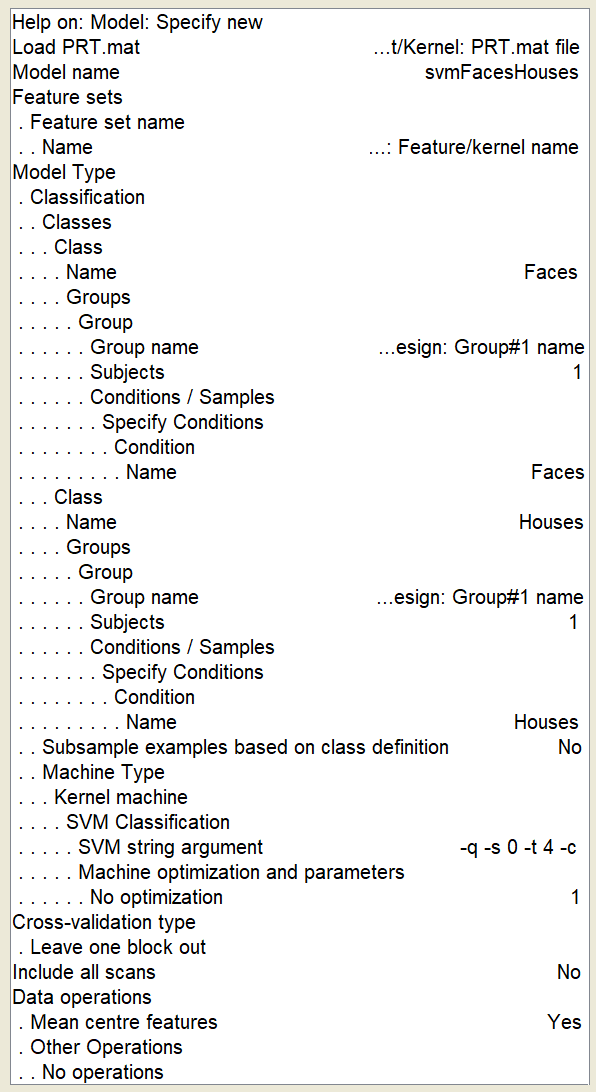
\includegraphics[scale=0.5]{images/Tutorial/v3/data_example1/batch_model_specify_new_full_final.png}
		\captionsetup{width=0.8\linewidth}
	\captionof{figure}{Final configuration of the `Model: Specify new' module}
	\label{fig:batch_model_specify_new_full_final}
\end{minipage}%
	\begin{minipage}[b][12.5cm][b]{0.5\textwidth}
  \centering
	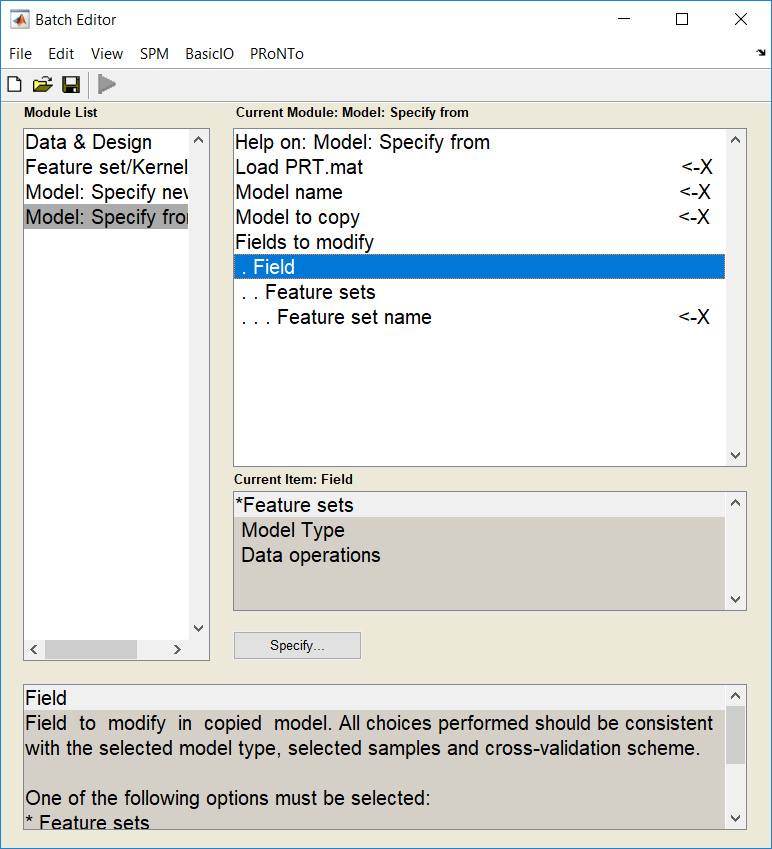
\includegraphics[scale=0.5]{images/Tutorial/v3/data_example1/batch_model_specify_from.png}
	\captionsetup{width=1\linewidth}
	\captionof{figure}{`Model: Specify from' module in {\tt matlabbatch}.}
    	\label{fig:batch_model_specify_from}
	\end{minipage}
\end{figure}

	\begin{figure}[h!]
	\centering
		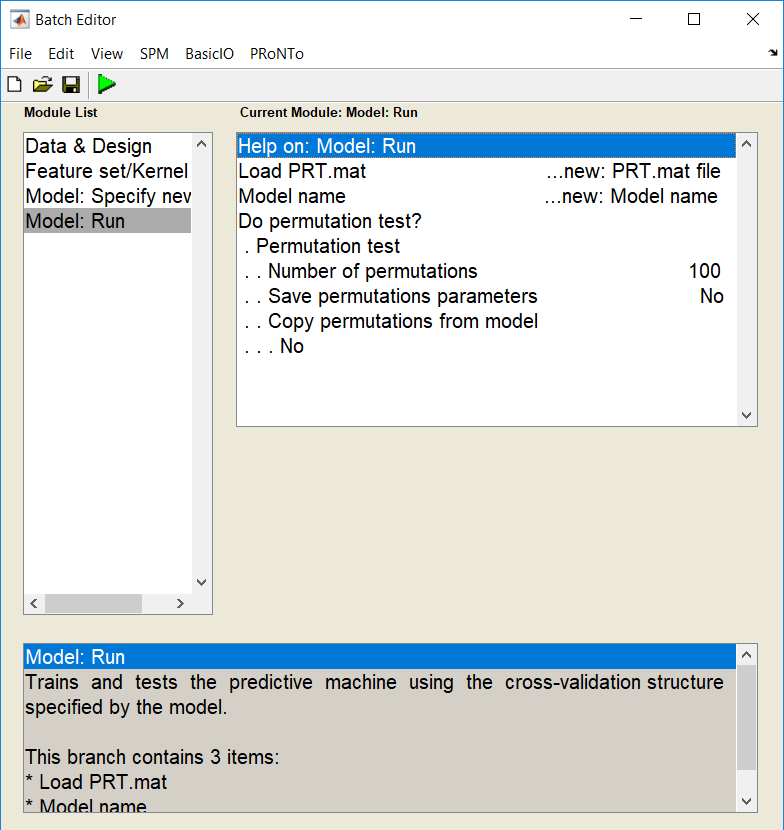
\includegraphics[scale=0.5]{images/Tutorial/v3/data_example1/batch_model_run_final.png}
	\caption{Final configuration of the `Model: Run' module in {\tt matlabbatch}.}
	\label{fig:batch_model_run_final}
\end{figure}

%----------------------------------------------------------


\subsection{Model: Specify from (optional step)}

\begin{itemize}

    \item Click on `Model: Specify from' option on PRoNTo's {\tt matlabbatch} menu. Figure \ref{fig:batch_model_specify_from} is the full drop-down list of options.
	
    \item The `Specify model from' module is similar to the `Specify model new' module, with the appropriate fields disabled to ensure comparability between models. As in the `Specify model new' module first with the `PRT.mat' file selected, click on `Dependency' button to associate the `PRT.mat' file created in the previous step, or alternatively either double-click on `Load PRT.mat' option or click on `Specify' button to browse where `PRT.mat' file was saved.
    
    \item Choose a `Model name', e.g. `gpFacesHouses', and then specify the name of an existing model from which the previous specifications will be loaded, here `svmFacesHouses'.
    
    \item There are three different options you can change in your new model. The feature set, the model type and the data operations. For further information regarding these options the user is referred to \ref{chap:ModelCrossV}.

\end{itemize}

%----------------------------------------------------------

\subsection{Model: Run}

\begin{itemize}

	\item Click on the `Model: Run' option on PRoNTo's {\tt matlabbatch} menu.
	
	\item  With the `Load PRT.mat' field selected, click on the `Dependency' button to associate the `PRT.mat' file created in the previous `Specify model' step.
	
	\item Select the model name from the `Model: Specify new' module with the `Dependency' button, or write it {\it exactly}, as previously defined in the `Model: Specify new' module, here `svmFacesHouses'.

	\item In the field `Do permutation test?', select `Permutation test' with 1000 repetitions, or as many as you can closer to 1000.
	
	\item Leave both `Save permutations parameters' and `Copy permutations from model' as they are, i.e. `No'. `Copy permutations from model' should be set to `Yes' if one wants to make sure the same permutations are run for the different models, this will enable applying statistical tests to compare the models. In that case the two models should have exactly the same samples in each fold and use the same cross-validation scheme.

\end{itemize}

Figure \ref{fig:batch_model_run_final} is the final configuration of the {\tt matlabbatch} `Model: Run' module.
%-----------------------------------------------------

\subsection{Compute weights (optional step)}

\begin{itemize}

	\item Click on the `Compute weights' option on PRoNTo's {\tt matlabbatch} menu.

	\item With `Load PRT.mat' field selected, click on the `Dependency' button to associate the `PRT.mat' file created in the previous `Run model' step.
	
	\item Select the model name from the `Model: Specify new' module with the `Dependency' button.
	
	\item It's optional to define a name for the image. 
	
	\item Leave the `Build weights images for permutations' field as it is, i.e. `No'. 

\end{itemize}

Finally, save the batch (e.g. as batch\_run\_all.m) and click on the `Run Batch' option, in the `File menu'. The batch file created can then be opened and edited for further analyses. The results will be the same as those obtained using the GUI (see Section \ref{display_results}  of this chapter). Please note that in this case the `Sample averaging (within block)' operation was not selected when specifying the model. In order to obtain the same results as before, the model has to use the same data operations.
\\

Figure \ref{fig:batch_compute_weights_final} is the final configuration of the {\tt matlabbatch} `Compute weights' module.

	\begin{figure}[h!]
	\centering
		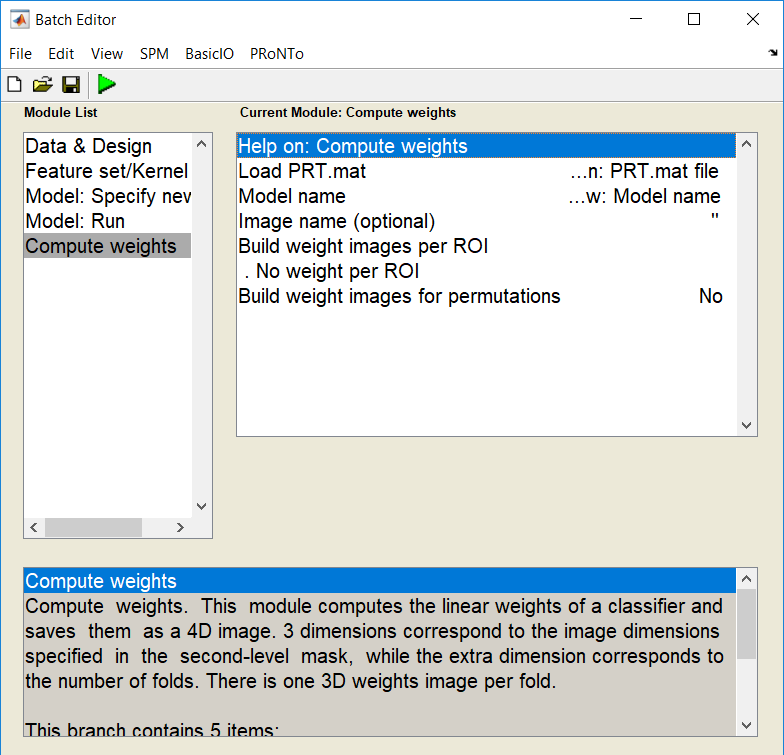
\includegraphics[scale=0.4]{images/Tutorial/v3/data_example1/batch_compute_weights_final.png}
	\caption{Final configuration of the `Compute weights' module in {\tt matlabbatch}.}
	\label{fig:batch_compute_weights_final}
\end{figure}











% \section{Multiclass classification (optional)}
% \label{sec:multiclass_classif}

% Another available functionality in PRoNTo is multiclass classification. This time we will use a kernal multiclass machine to try to predict 3 classes, faces, houses and cats. In order to do that the main module that needs changing is the `Model: Specify new', where instead of 2 classes we will have to input 3 classes, and also include a multiclass machine instead of the Binary SVM machine we used previously.

% \begin{itemize}
	
% 	\item Select the `PRT.mat' file and provide a name to the model, e.g. `gpFacesHousesCats'.

% 	\item Select the `HaxbyFeatures' feature set.

% 	\item	Leave the option `Use kernels' tick box as it is, i.e. `Yes'.

% 	\item	Select the `Classification' model type and click on `Define classes' button. A new window will open, `Specify classes' (Figure \ref{fig:gui_specify_new_specify_classes}), to define the number of classes and a name for each class. We will define 3 classes. First click `Class 1' on the tab `Class'. For `Class 1' select subject `S1' and the condition `Faces'. Similarly for `Class 2' and `Class 3' select subject `S1' for both, and the conditions `Houses' and `Cats' respectively. Leave the `Subsample according to smallest class' as it is for now. Once you have appropriately specified everything, click `Done'.
	
% 	\item Select the `Multiclass GPC' option, in the `Machine' field.
	
% 	\item Leave the option `Optimize hyper-parameter' tick box unchecked and `Cross-Validation Scheme' (internal loop) as it is. 
	
% 	\item Select the `k-fold CV on Block' cross-validation scheme (external loop) with k=5.
	
% 	\item In the `Data operations' box, select only the `Mean centre features using training data' option.
	
% 	\item As previously, click `Specify and run model' and the model will be immediately estimated, albeit with no permutations.

% \end{itemize}

% Opening up the `Display Results' module and clicking at our newly-built multiclass model you will see that a few small things are different. For example we now have 3 class accuracies (CA) instead of 2, one for each class. Furthermore, if you click in one specific fold you will notice that the histogram of this fold has 3 curves, again one for each class.

%--------------------------------------------------------------------